%%%%%%%%%%%%%%%%%%%%%%%%%%%%%%%%%%%%%%%%%%%%%%%%%%%%%%%%%%%%%%%%%%%%%%%%%%%%%%%%
% DUET ICRA 2026 draft.
% Based on the official Papercept ieeeconf template downloaded from:
% https://ras.papercept.net/conferences/support/files/ieeeconf.zip
%%%%%%%%%%%%%%%%%%%%%%%%%%%%%%%%%%%%%%%%%%%%%%%%%%%%%%%%%%%%%%%%%%%%%%%%%%%%%%%%

\documentclass[letterpaper, 10 pt, conference]{ieeeconf}

\IEEEoverridecommandlockouts
\overrideIEEEmargins

\usepackage{amsmath}
\usepackage{amssymb}
\usepackage{booktabs}
\usepackage{colortbl}
\usepackage{xcolor}
\usepackage{graphicx}
\usepackage{multirow}
\usepackage{url}
\usepackage{capt-of}

\title{\LARGE \bf
DUET: Endogenous Failure Detection and Recovery via Dual-Action Manifold Alignment
}

\author{Anonymous Authors% <-this % stops a space
\thanks{This paper is an ICRA 2026 draft. Author names and affiliations are omitted for anonymous review.}
}

\begin{document}

\maketitle
\thispagestyle{empty}
\pagestyle{empty}

\begin{abstract}
Vision-language-action (VLA) policies map visual observations and language instructions to robot actions but can drift from successful behavior during closed-loop execution, raising the risk of task failure. We focus on recoverable execution deviations---where the rollout has left the demonstrated support yet retrying remains feasible---rather than irreversible failures requiring replanning. Existing solutions decouple detection and recovery into separate modules, often requiring human takeover data. We introduce DUET, a backbone-agnostic dual-action-head module that predicts relative actions for smooth nominal control and absolute waypoints for trajectory re-entry. Disagreement between the two action spaces signals rising failure risk, while the absolute waypoint supplies the retry direction. Asymmetric training keeps the relative branch sensitive to deviations and the absolute branch robust to visual disturbances. The module interfaces with shared vision-language features and can be attached to different VLA backbones. On LIBERO, DUET improves nominal success from $93.8\%$ to $96.9\%$ and action-perturbation success from $27.9\%$ to $64.6\%$ over its relative-only head. A controlled Franka protocol on a separately trained $\pi_0$ backbone is specified to test physical retry; its results remain pending.
\end{abstract}

\begin{figure*}[t]
\centering
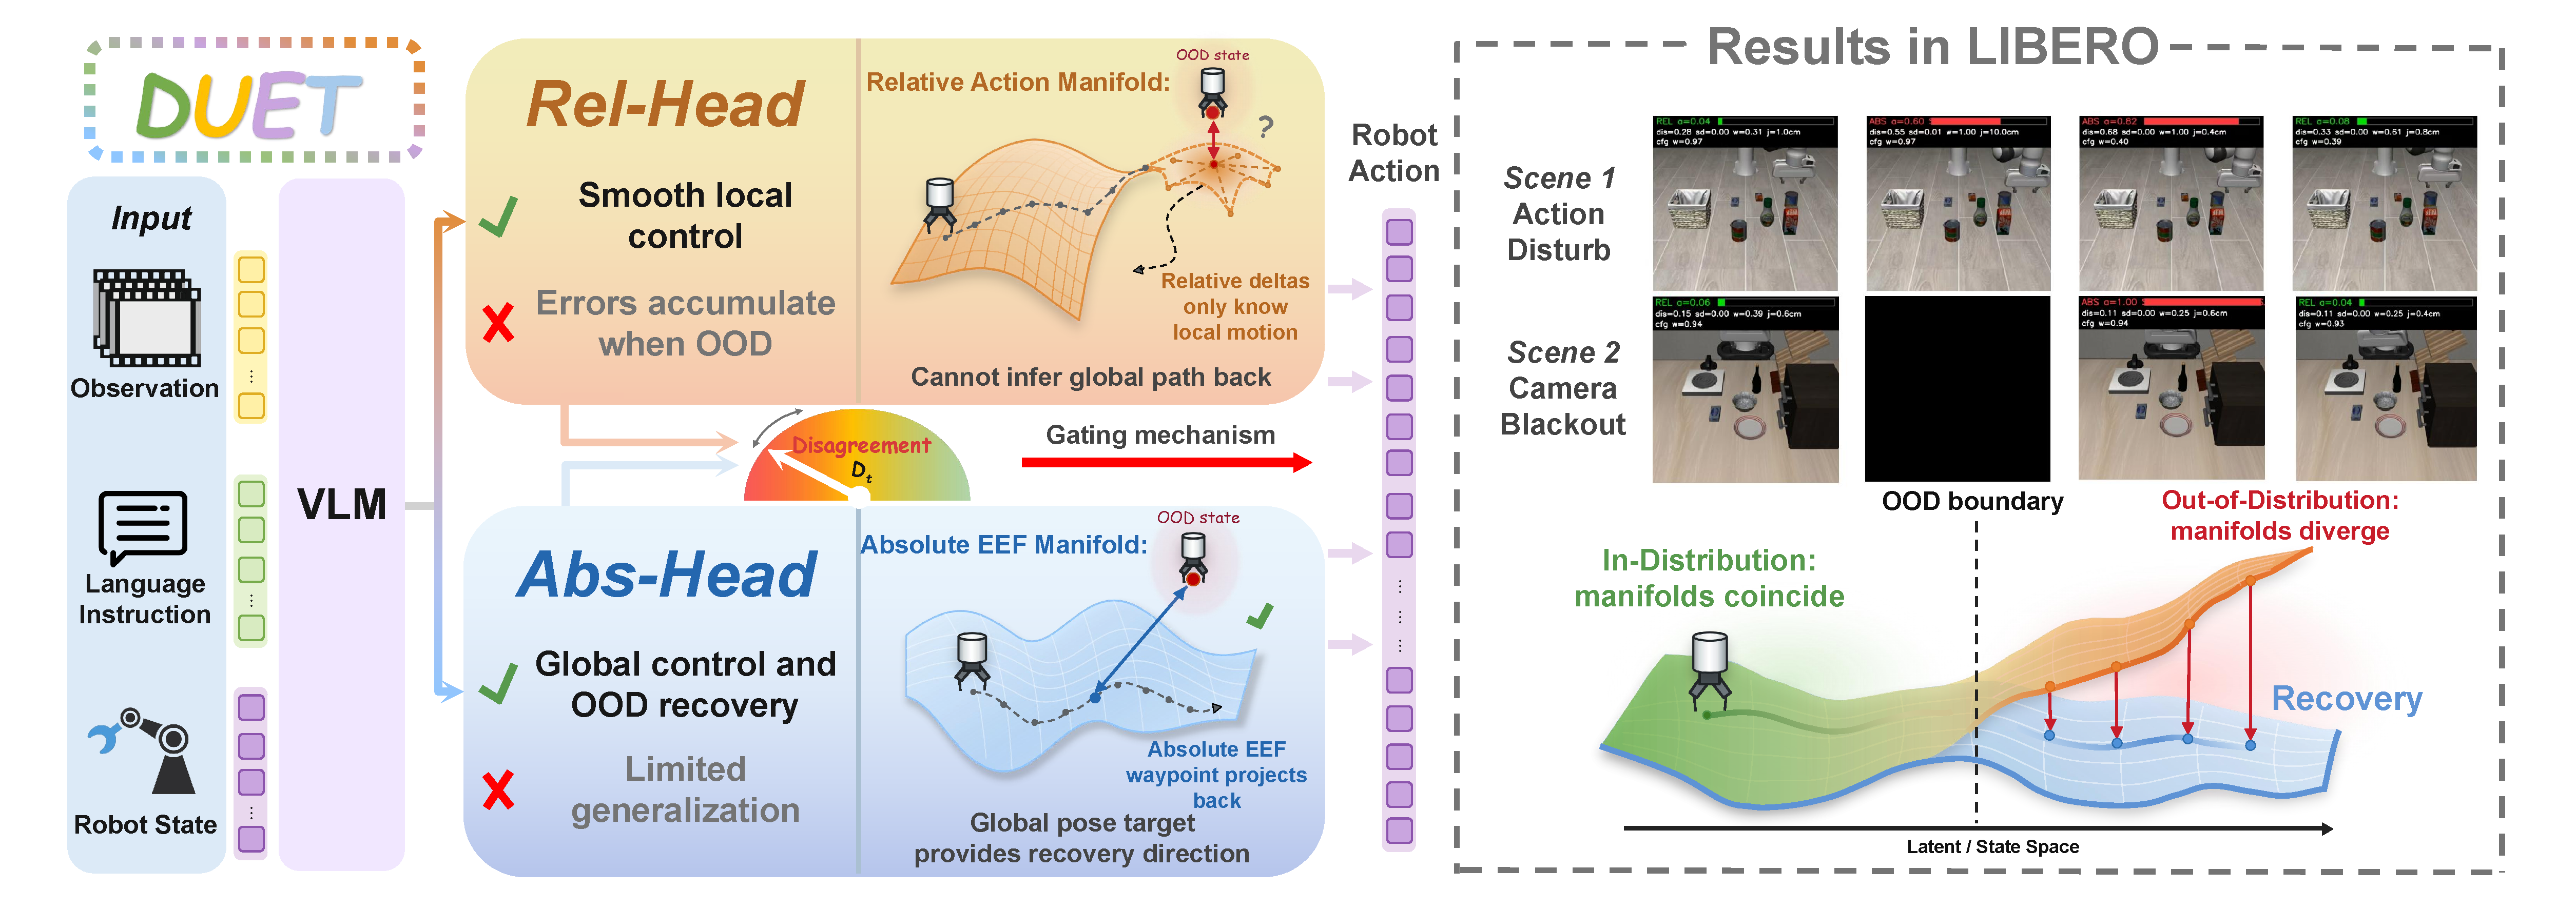
\includegraphics[width=0.96\textwidth]{figures/fig1.pdf}
\caption{Failure-aware retry with dual action spaces. Relative and absolute predictions agree during nominal execution but diverge when a recoverable deviation drives the rollout OOD, exposing an endogenous disagreement score $D_t$. Relative actions provide precise local motion, whereas absolute waypoints bring the robot back toward a demonstrated execution path for retry.}
\label{fig:teaser}
\end{figure*}

\section{INTRODUCTION}

Vision-language-action (VLA) policies adapt pretrained vision-language models to map visual observations and language instructions to robot actions \cite{rt2,openvla,starvla}. Trained exclusively on successful demonstrations, they can drift during closed-loop execution until the rollout can no longer reliably complete the task---an \emph{execution failure}. Before that outcome becomes irreversible, the robot may already have departed from the observations, configurations, or action consequences represented by successful demonstrations. We call this intermediate condition an \emph{execution deviation}: the rollout has left the support of demonstrated success, raising failure risk. Deviation and failure are related but not equivalent---an unseen state may still be handled successfully, while failures can also arise from compounding errors within seemingly familiar observations. Our focus is the practical regime in which a deviation has elevated failure risk but the task can still be completed by returning toward demonstrated behavior.

To address this problem, existing methods typically require two additional training stages. First, they train an external failure-prediction model to recognize when the policy is leaving the support of successful behavior \cite{faildetect}. They then collect a large set of recovery trajectories---often through human takeovers or expert interventions---to train a separate controller that brings the robot back \cite{dagger,sirius,intervengen}. The detector and recovery policy are therefore trained with different supervision and remain loosely coupled: the former only raises an alarm, while the latter depends on costly data collected after failures occur. We ask whether a VLA can use its own action predictions to detect a recoverable execution deviation and generate a retry direction from successful demonstrations alone, without an external failure model or recovery data.

Achieving this without an external failure predictor or additional recovery data poses two coupled challenges. Successful demonstrations teach a policy how to act along successful trajectories, but do not explicitly teach it when its actions become unreliable or how to return after leaving those trajectories. Detection must therefore derive a meaningful risk signal from the policy itself, while recovery must infer a corrective direction from demonstrations that do not cover the encountered deviation. Our approach is motivated by a recurring observation from our extensive prior experiments: with large-scale training data, relative actions often yield the best performance by enabling stronger generalization. However, after fine-tuning on a small demonstration set, relative-action policies struggle to recover autonomously once execution enters out-of-distribution states. Absolute actions exhibit the complementary tradeoff: they generalize less effectively in the large-data regime but more readily guide execution back toward demonstrated behavior after a deviation under limited-data fine-tuning. This observation motivates DUET, which combines a relative head for nominal execution with an absolute head for trajectory re-entry. Disagreement between the relative action and the correction toward the absolute waypoint signals a recoverable deviation, while the waypoint itself supplies a retry direction.

The module attaches to the backbone's shared vision-language representation without changing its architecture or pretraining. We train it on StarVLA \cite{starvla} in simulation and $\pi_0$ (OpenPi) \cite{pi0} for real-robot deployment.

At inference, a soft gate shifts from relative control toward the waypoint correction as disagreement rises, then returns after realignment. DUET addresses recoverable deviations; irreversible failures, hardware faults, and cases requiring a new task strategy remain outside its scope.

Our contributions are threefold:
\begin{itemize}
    \item We formulate failure-aware retry as detecting recoverable execution deviations from successful behavior and re-entering its support. Cross-space disagreement between relative and absolute action heads serves as an endogenous failure-risk signal requiring no failure labels, outperforming dedicated detectors on TPR and AUROC (\S\ref{sec:detection}).
    \item We propose DUET, a dual-action-head VLA in which the same disagreement that detects deviations simultaneously provides the waypoint-based recovery direction, unifying detection and correction in a single mechanism while preserving smooth nominal control (\S\ref{sec:nominal}, \S\ref{sec:retry}).
    \item We evaluate DUET on StarVLA in LIBERO simulation (\S\ref{sec:retry}) and define a matched clean/disturbed protocol on a separately trained $\pi_0$ (OpenPi) controller across four Franka tasks (\S\ref{sec:real_robot}) to test the design's applicability across backbones.
\end{itemize}


\section{RELATED WORK}

\subsection{Failure Detection for Robot Policies}
Runtime failure detection estimates whether a policy remains within the support of successful behavior. Diff-DAgger uses diffusion uncertainty to request intervention \cite{diffdagger}; Sentinel monitors action inconsistency and task progress \cite{sentinel}. FAIL-Detect formulates failure detection as sequential OOD testing on successful executions \cite{faildetect}; FIPER combines representation novelty with action uncertainty \cite{fiper}.

VLA-specific methods use internal features or external foundation models. SAFE learns a detector from successful and failed rollouts \cite{safe}; AHA trains a VLM to detect and diagnose failures \cite{aha}. All of these methods---including FAIL-Detect's logpZO \cite{faildetect}---produce a scalar alarm but no recovery action. DUET instead detects execution deviations through disagreement between two action spaces; the same inconsistency that signals rising failure risk provides the waypoint-based recovery direction, coupling detection and correction without additional supervision.

\subsection{Recovery from Execution Failures}
Recovery methods commonly expand the training distribution with expert corrections. DAgger queries experts on policy-induced states \cite{dagger}; intervention-based methods collect human takeovers \cite{eil,sirius}; IntervenGen transforms limited interventions into corrective trajectories \cite{intervengen}. These reduce compounding errors but require additional recovery data.

Foundation-model systems use semantic supervisors. RACER learns from language-annotated recovery trajectories \cite{racer}; AHA and VLM controllers diagnose failures and guide correction \cite{aha,vlmrecovery}. In all cases detection and recovery remain separately trained or prompted. DUET couples both without extra data: absolute states from successful demonstrations serve as recovery anchors, and cross-space disagreement determines when and how strongly to move toward them.

\section{METHOD}
\label{sec:method}

\subsection{Dual Action Spaces and Architecture}
DUET predicts demonstrated behavior in complementary coordinates: relative actions specify local motion from the measured pose, while absolute waypoints retain a scene-conditioned reference. Given images $o_t$, instruction $l$, and proprioceptive state $s_t$, the heads output chunks over a horizon $K$:
\begin{equation}
\begin{aligned}
    \hat{\Delta A}_t &= f_{\mathrm{rel}}(o_t,l,s_t)
    \in \mathbb{R}^{K\times 7}, \\
    \hat{W}_t &= f_{\mathrm{abs}}(o_t,l)
    \in \mathbb{R}^{K\times 7}.
\end{aligned}
\end{equation}
Commands decompose as $a_t=[a_{p,t},a_{g,t}]$, with six pose dimensions $a_{p,t}$ and one gripper dimension $a_{g,t}$. Relative outputs are operational-space-control deltas; absolute outputs encode matched future poses and gripper states in the absolute frame. Only pose commands are fused; the discrete open/close decision remains with the relative head.

\begin{figure}[!t]
\centering
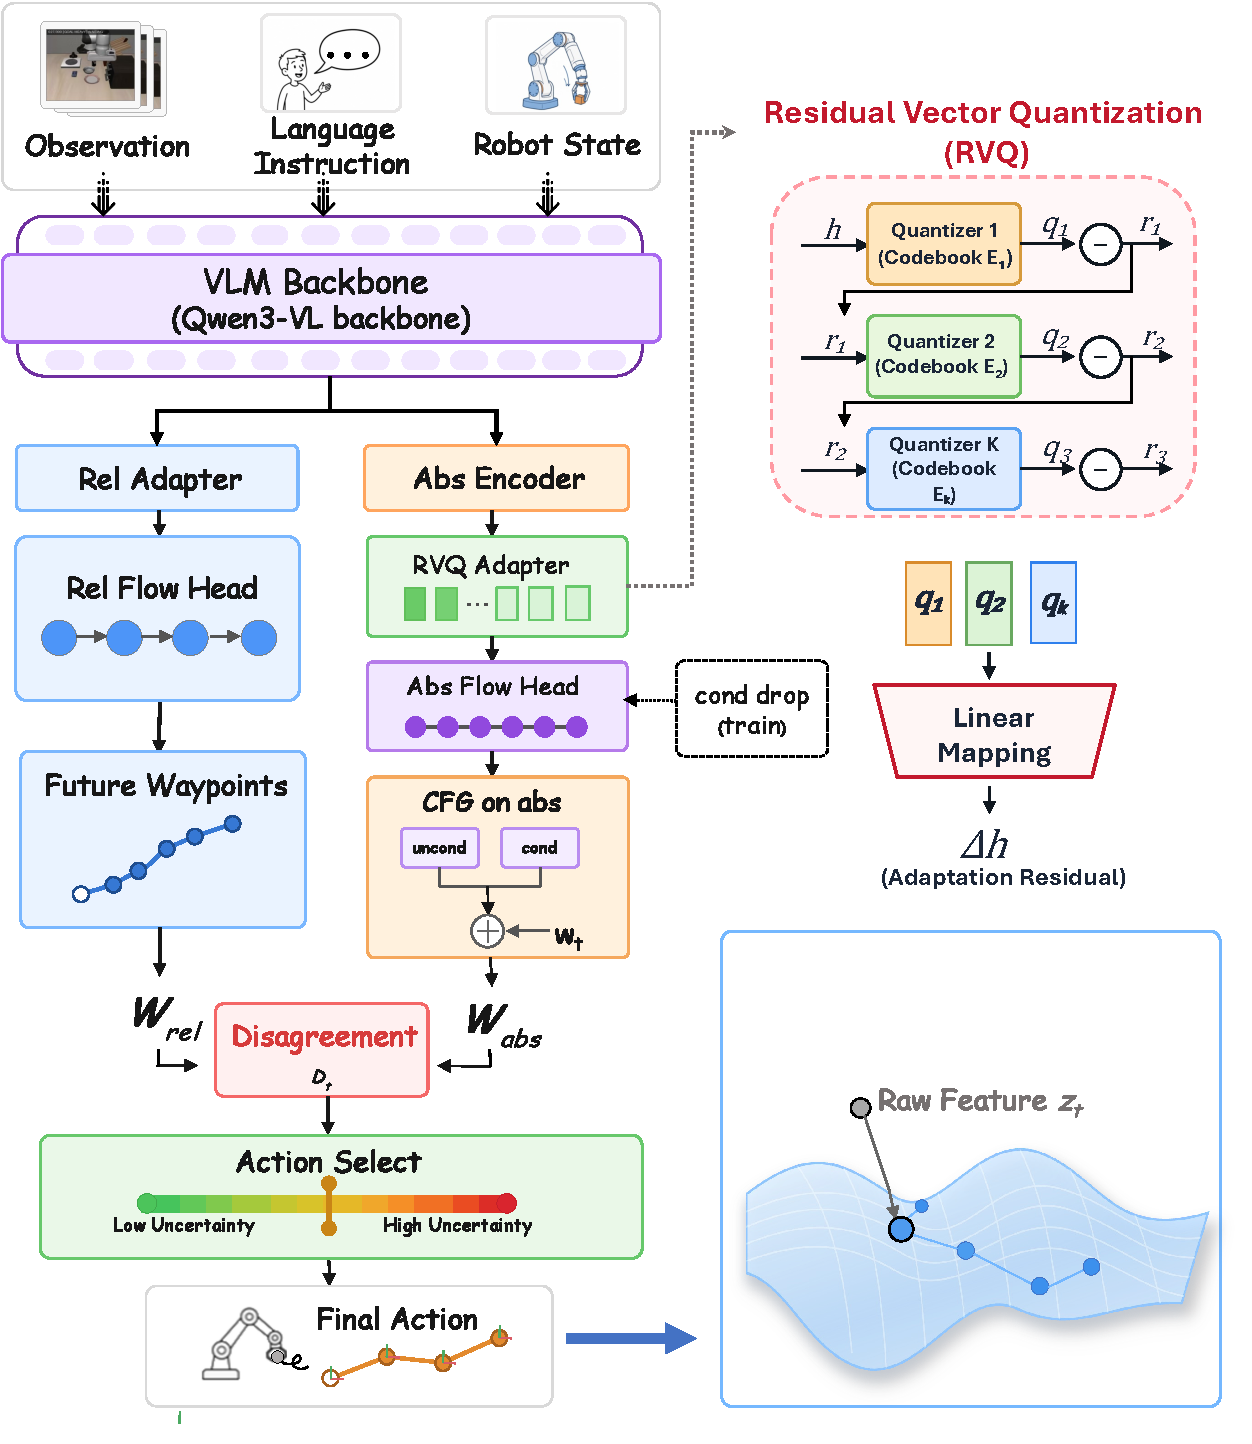
\includegraphics[width=\columnwidth]{figures/fig2.pdf}
\caption{DUET combines a shared encoder with state-aware relative and RVQ-conditioned absolute heads. Their disagreement guides OOD detection and closed-loop waypoint retry.}
\label{fig:architecture}
\end{figure}

We model successful end-effector trajectories as a manifold $\mathcal{M}_l\subset SE(3)$. Near it, relative commands describe local tangent motion in $T_{p_t}\mathcal{M}_l$, while absolute waypoints reference global coordinates on $\mathcal{M}_l$. After a deviation, the relative head continues from the displaced pose, whereas the absolute head preserves a demonstrated target. Transporting that waypoint to the live pose makes the predictions comparable: they align when local continuation agrees with the reference and can separate off-support. This interpretation motivates detection but does not imply that every failure produces disagreement.

Both heads share a VLM encoder (Fig.~\ref{fig:architecture}) but use asymmetric conditioning. The relative head attends to the full hidden sequence and receives $s_t$ through a state encoder. The absolute head excludes explicit proprioception; state tokens follow visual-language tokens in the causal encoder and are omitted from its pooling. This prevents the live pose from being copied into the reference while preserving shared task semantics.

\subsection{Disagreement-Preserving Learning}
Each successful demonstration supplies synchronized delta actions and normalized future poses, so the heads learn the same chunk in different coordinates without failure labels or takeover actions. We optimize their flow-matching losses \cite{pi0} with an RVQ commitment loss, but omit cross-head consistency supervision that could suppress later detection evidence. RVQ quantizes pooled state-free visual-language features into a discrete atlas of demonstrated task phases, anchoring absolute predictions to successful behavior \cite{vqvae,rvq}; its residual is retained only as auxiliary telemetry.

Asymmetric augmentation preserves this division of labor. The absolute head and RVQ see clean and perturbed observations, making the reference robust to visual corruption; relative-head loss is computed only on clean samples, keeping local control tied to demonstrations and deviations visible as mismatch. For classifier-free guidance (CFG) \cite{cfg}, condition dropout replaces absolute-head conditions with learned null tokens to learn conditional and marginal waypoint flows.

\subsection{Endogenous OOD Detection and Retry}
Both branches are unnormalized before comparison in the tangent coordinates of the live pose. For live pose $p_t=(x_t,R_t)$ and predicted waypoint $\hat{w}_{p,t}=(\hat{x}_t,\hat{R}_t)$, the waypoint-induced retry direction is
\begin{equation}
    c_t=\operatorname{clip}\!\left(
    \begin{bmatrix}
    (\hat{x}_t-x_t)/\sigma_p \\
    \operatorname{Log}(\hat{R}_tR_t^{-1})/\sigma_R
    \end{bmatrix},-1,1\right),
    \label{eq:recovery_vector}
\end{equation}
where $\operatorname{Log}$ denotes the three-vector rotation logarithm and $\sigma_p,\sigma_R$ convert pose error into action units. Comparing it with the relative pose command $\hat{\delta a}_{p,t}$ gives endogenous OOD evidence:
\begin{equation}
    D_t=\frac{\left\|c_t-
    \operatorname{clip}(\hat{\delta a}_{p,t},-1,1)\right\|_2}{\sqrt{6}}.
    \label{eq:disagreement}
\end{equation}
The comparison produces both quantities needed for retry: $D_t$ is scalar detection evidence, while $c_t$ is its six-dimensional correction direction. The auxiliary $S_t$ averages coordinatewise distances outside the training pose bounds, normalized by each coordinate's training range. The control score $q_t$ and fusion weight are
\begin{equation}
\begin{aligned}
    q_t &= D_t + \lambda S_t, \\
    \alpha_t &= \sigma(k(q_t-\tau)).
\end{aligned}
\end{equation}
Here $\sigma$ is the sigmoid, $k$ its slope, $\tau$ the switching threshold, and $\lambda$ the state-distance weight. Low $q_t$ preserves relative control; rising inconsistency smoothly increases the absolute correction. The executed command is
\begin{equation}
\begin{aligned}
    a_{p,t} &= (1-\alpha_t)\hat{\delta a}_{p,t} + \alpha_t c_t, \\
    a_{g,t} &= \hat{\delta a}_{g,t}.
\end{aligned}
    \label{eq:fused_action}
\end{equation}
CFG strength follows $w_t=w_{\max}-(w_{\max}-w_{\min})\alpha_{t-1}$ for the next chunk. When the trajectory remains feasible, rising disagreement shifts control toward $c_t$ for retry; realignment lowers the gate and restores relative execution. The same signal therefore invokes and terminates correction.

\section{EXPERIMENTS}

% Place the two wide overview tables before the experiment text so that they
% can be scheduled at the top of the next page, close to their first citations.
\begin{table*}[!t]
\caption{Execution-failure protocols and their correspondence to the introduction.}
\label{tab:ood_taxonomy}
\centering
\resizebox{0.96\textwidth}{!}{%
\begin{tabular}{llll}
\toprule
Family & Protocol & What becomes OOD & Introduction example \\
\midrule
Action execution & Action perturbation & Induced trajectory / command-to-motion map & Execution drift after locally plausible commands \\
Robot displacement & EEF teleport & Robot-arm pose & Unexpected displacement of the robot arm \\
Object / grasp & Vertical grasp drop & Robot--object configuration & Dropped object or failed hold \\
Visual occlusion & Camera blackout & Current visual observation & Transient occlusion \\
Contact / scene & External force & Robot--world interaction & External disturbance during contact \\
\bottomrule
\end{tabular}}
\end{table*}

\begin{table*}[!t]
\caption{Failure-detection comparison under matched protocols. TPR, TNR, balanced accuracy (Bal.-Acc.), AUROC, and Loc.@16 are higher-is-better; detection delay is lower-is-better. Bold values indicate the best result in each column.}
\label{tab:detector_baselines}
\centering
\resizebox{0.96\textwidth}{!}{%
\begin{tabular}{lccccccc}
\toprule
Method & TPR $\uparrow$ & TNR $\uparrow$ & Bal.-Acc. $\uparrow$ & AUROC $\uparrow$ & Delay (steps) $\downarrow$ & Delay (s) $\downarrow$ & Loc.@16 $\uparrow$ \\
\midrule
\rowcolor{gray!20}
DUET & \textbf{0.900} & 0.265 & 0.582 & \textbf{0.845} & 28.3 & 1.41 & 0.523 \\
logpZO~\cite{faildetect} & 0.889 & 0.243 & 0.566 & 0.817 & 22.7 & 1.14 & \textbf{0.569} \\
RND~\cite{rnd,faildetect} & 0.842 & \textbf{0.361} & \textbf{0.602} & 0.549 & 26.1 & 1.31 & 0.330 \\
PCA-kmeans~\cite{faildetect} & 0.884 & 0.283 & 0.583 & 0.625 & \textbf{20.3} & \textbf{1.01} & 0.503 \\
STAC~\cite{sentinel} & 0.839 & 0.311 & 0.575 & 0.494 & 25.8 & 1.29 & 0.260 \\
\bottomrule
\end{tabular}}
\end{table*}

We organize the experiments around three questions:
\begin{itemize}
    \item[\textbf{(Q1)}] \textbf{Endogenous OOD detection:} Can DUET identify execution states that are inconsistent with successful behavior using only successful demonstrations?
    \item[\textbf{(Q2)}] \textbf{Nominal execution:} Does the dual-action mechanism preserve normal task execution?
    \item[\textbf{(Q3)}] \textbf{Failure-aware retry:} When an OOD deviation remains recoverable, can DUET use its detected inconsistency to re-enter successful behavior and complete the task?
\end{itemize}
We use matched LIBERO trials, controlled disturbances, detector analysis, component ablations, and a real-robot protocol, reporting detection, nominal success, and closed-loop retry separately.

\subsection{Evaluation Protocol}
We evaluate on four LIBERO suites \cite{libero}---Spatial, Object, Goal, and LIBERO-10---with $10$ tasks and $50$ initial states per task ($500$ episodes per suite). Three methods are compared:
\begin{itemize}
    \item \emph{StarVLA}~\cite{starvla}: relative-action-only VLA trained with the same data and budget but without the absolute head (external baseline).
    \item \emph{DUET-Rel}: relative head of the dual-action checkpoint with $\alpha_t{=}0$ (isolates co-training from fusion).
    \item \emph{DUET}: full adaptive controller (Eq.~\eqref{eq:fused_action}).
\end{itemize}
StarVLA $\to$ DUET-Rel measures co-training; DUET-Rel $\to$ DUET isolates retry. Within each pair, architecture, data, task, initial state, and perturbation are fixed. Simulation uses StarVLA; the Franka study (\S\ref{sec:real_robot}) uses a separately trained $\pi_0$ (OpenPi) \cite{pi0} with the same module and fusion logic, testing cross-backbone applicability rather than zero-shot transfer.

Perturbations use a fixed policy step and deterministic seeds. DUET and DUET-Rel share $(\mathrm{task},\mathrm{initial\ state})$ keys; paired success is assessed with McNemar $p$-values. For semantic preconditions (e.g., grasp drop requires a held object), we report injection coverage and retain uninjected episodes. Table~\ref{tab:ood_taxonomy} maps protocols to failure types; heterogeneous disturbances are not pooled.

\subsection{\textbf{(Q1)} Endogenous OOD Detection}
\label{sec:detection}
To answer \textbf{Q1}, Table~\ref{tab:detector_baselines} compares cross-space disagreement $D_t$ with success-only detectors from FAIL-Detect \cite{faildetect} and STAC \cite{sentinel} under matched protocols.

DUET improves detection discrimination while keeping detection delay close to prior methods: $1.41$\,s versus $1.01$--$1.31$\,s. It achieves the highest AUROC ($0.845$), exceeding the strongest baseline, logpZO ($0.817$), and substantially outperforming RND, PCA-kmeans, and STAC ($0.494$--$0.625$). DUET also attains the highest TPR ($0.900$), although its balanced accuracy is not the best. These results show that disagreement between the two action spaces identifies execution deviations without failure labels, with improved ranking quality at a modest additional delay.


\subsection{\textbf{(Q2)} Nominal Execution}
\label{sec:nominal}
\textbf{Q2} asks whether failure-aware retry preserves ordinary execution when no disturbance is injected. DUET attains $96.9\%$ average success (Table~\ref{tab:benchmark}), matching the reported $\pi_{0.5}$ result. External rows serve as benchmark context only; the controlled comparison is DUET versus DUET-Rel on the same checkpoint. Adaptive fusion raises the average from $93.8\%$ to $96.9\%$, with the largest lifts on Goal ($+5.6$) and LIBERO-10 ($+5.8$). Even without injected perturbation, rollouts can drift from the demonstrated support; the absolute waypoint provides a return target that the relative-only controller lacks.

\begin{table}[t]
\caption{Nominal task success (\%) on LIBERO. External rows are reported results and are included only for benchmark context. StarVLA uses joint $30$k training; DUET uses suite-specific $10$k checkpoints.}
\label{tab:benchmark}
\centering
\resizebox{\columnwidth}{!}{%
\begin{tabular}{lccccc}
\toprule
Method & Spatial & Object & Goal & LIBERO-10 & Avg. \\
\midrule
$\pi_{0.5}$ (reported) & 98.8 & 98.2 & 98.0 & 92.4 & 96.9 \\
StarVLA-GR00T (reported) & 97.8 & 98.8 & 97.4 & 92.0 & 96.5 \\
\midrule
\rowcolor{gray!20}
DUET & 98.8 & 99.4 & 97.6 & 91.8 & 96.9 \\
DUET-Rel & 98.0 & 99.2 & 92.0 & 86.0 & 93.8 \\
\bottomrule
\end{tabular}}
\end{table}

\begin{table*}[!t]
\caption{Closed-loop success (\%) under four disturbance families ($N{=}500$ per cell). Overall rows aggregate medium and severe results across all four suites. Per-suite Rel$\to$DUET $\Delta$ has McNemar $p{<}10^{-3}$ except teleport/Spatial (medium $p{=}0.21$, severe $p{=}0.067$) and blackout/Object medium.}
\label{tab:ood_detailed}
\centering
\footnotesize
\begin{tabular*}{\textwidth}{@{\extracolsep{\fill}} l cccc @{\hspace{1.2em}} cccc @{}}
\toprule
& \multicolumn{4}{c}{Medium} & \multicolumn{4}{c}{Severe} \\
\cmidrule(lr){2-5}\cmidrule(l){6-9}
Suite & StarVLA & Rel. & DUET & $\Delta$ & StarVLA & Rel. & DUET & $\Delta$ \\
\midrule
\multicolumn{9}{@{}l}{\textit{(i) Action perturbation (step $5$)}} \\
Spatial    & 60.0 & 54.0 & 74.0 & $+20.0$ & 14.0 & 12.8 & 43.2 & $+30.4$ \\
Object     & 41.6 & 48.8 & 84.4 & $+35.6$ &  7.8 &  7.8 & 60.6 & $+52.8$ \\
Goal       & 52.2 & 47.2 & 74.2 & $+27.0$ & 18.8 & 10.6 & 52.6 & $+42.0$ \\
LIBERO-10  & 36.2 & 36.6 & 78.6 & $+42.0$ &  6.2 &  5.4 & 49.0 & $+43.6$ \\
\textbf{Overall} & 29.6 & \textbf{27.9} & \textbf{64.6} & $\mathbf{+36.7}$ & \multicolumn{4}{c}{\textit{med$+$sev combined}} \\
\midrule
\multicolumn{9}{@{}l}{\textit{(ii) EEF teleport (step $39$)}} \\
Spatial    & 55.4 & 54.6 & 57.6 & $+3.0$  & 46.8 & 48.2 & 52.6 & $+4.4$ \\
Object     & 43.4 & 36.2 & 76.0 & $+39.8$ & 21.2 & 20.8 & 68.4 & $+47.6$ \\
Goal       & 41.6 & 33.4 & 52.4 & $+19.0$ & 30.4 & 28.2 & 50.6 & $+22.4$ \\
LIBERO-10  & 40.4 & 35.8 & 60.8 & $+25.0$ & 21.4 & 18.4 & 56.8 & $+38.4$ \\
\textbf{Overall} & 37.6 & \textbf{34.5} & \textbf{59.4} & $\mathbf{+24.9}$ & \multicolumn{4}{c}{\textit{med$+$sev combined}} \\
\midrule
\multicolumn{9}{@{}l}{\textit{(iii) Vertical grasp drop (Object only, medium, step $67$)}} \\
Object     & 90.6 & 89.2 & \textbf{95.2} & $\mathbf{+6.0}$  & \multicolumn{4}{c}{---} \\
\midrule
\multicolumn{9}{@{}l}{\textit{(iv) Camera blackout (step $23$)}} \\
Spatial    & 81.0 & 88.0 & 94.4 & $+6.4$  & 42.4 & 63.2 & 95.2 & $+32.0$ \\
Object     & 91.8 & 98.6 & 96.8 & $-1.8$  & 64.2 & 95.0 & 97.2 & $+2.2$ \\
Goal       & 65.4 & 86.0 & 86.4 & $+0.4$  & 35.4 & 65.8 & 85.8 & $+20.0$ \\
LIBERO-10  & 60.0 & 65.6 & 84.2 & $+18.6$ & 24.4 & 25.6 & 86.2 & $+60.6$ \\
\textbf{Overall} & 58.1 & \textbf{73.5} & \textbf{90.8} & $\mathbf{+17.3}$ & \multicolumn{4}{c}{\textit{med$+$sev combined}} \\
\bottomrule
\end{tabular*}
\end{table*}

\subsection{\textbf{(Q3)} Failure-Aware Retry under Execution Disturbances}
\label{sec:retry}
\textbf{Q3} asks whether DUET can complete a feasible task after an OOD execution deviation. Across the four primary disturbance protocols in Table~\ref{tab:ood_detailed}, the answer is yes at the aggregate level. Compared with DUET-Rel, DUET raises success from $27.9\%$ to $64.6\%$ under action perturbation ($+36.7$ pp), from $34.5\%$ to $59.4\%$ after EEF teleport ($+24.9$ pp), from $89.2\%$ to $95.2\%$ after grasp drop ($+6.0$ pp; coverage $\geq 98.8\%$), and from $73.5\%$ to $90.8\%$ during camera blackout ($+17.3$ pp). DUET also exceeds StarVLA in all four protocols.


\begin{figure}[t]
\centering
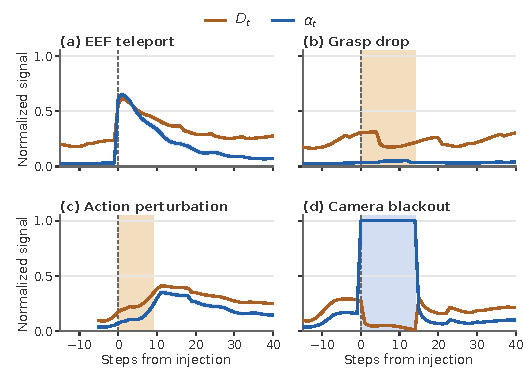
\includegraphics[width=\columnwidth]{figures/fig_ood_mechanism_grid.pdf}
\caption{Controller dynamics on the Object suite under (a) end-effector teleport, (b) vertical grasp drop, (c) action perturbation, and (d) camera blackout. Traces are aligned to the actual injection time and show means with pointwise bootstrap 95\% confidence intervals over successfully injected episodes. Shading denotes the perturbation or forced-hold window.}
\label{fig:ood_mechanism_grid}
\end{figure}

The largest gains occur under action perturbation and EEF teleport, where displaced relative control lacks a return target; the smaller grasp-drop gain reflects the strong relative-only baseline. The improvement is not universal at the cell level: DUET is $1.8$ pp below DUET-Rel for medium camera blackout on Object, and the Spatial teleport gains are not statistically significant. Figure~\ref{fig:ood_mechanism_grid} shows the retry mechanism: after a disturbance, disagreement raises $\alpha_t$ and shifts pose control toward the absolute waypoint; after re-entry, $\alpha_t$ falls and relative control resumes. In a supplementary contact-force check, DUET improves success from $92.22\%$ to $95.95\%$ ($+3.73$ pp), indicating that adaptive fusion remains stable in contact-rich tasks. Together, these results show that cross-space inconsistency can both trigger and guide a successful retry, directly answering \textbf{Q3}.

\subsection{Ablations}
\label{sec:ablations}
Table~\ref{tab:ablations} separates inference-time controls from training-time replacements. Disabling the absolute branch (DUET-Rel) accounts for all reported gains; fixing CFG at $w{=}1$ leaves performance unchanged, so the benefit comes from the waypoint itself. Absolute-only ($\alpha_t{=}1$) and fixed-fusion ($\alpha_t{=}0.5$) controls collapse performance, confirming the disagreement gate is essential. Training ablations (RVQ $\to$ MLP, symmetric augmentation, state-aware absolute head) are preregistered as TODO.

\paragraph{Fusion weight on clean trajectories.}
Across $2{,}000$ clean episodes, the mean $\alpha_t$ is TODO, the $95^{\mathrm{th}}$ percentile is TODO, and only TODO\% of steps exceed $0.5$---confirming that the fusion weight stays near zero during nominal execution.

\paragraph{Sensitivity to $\tau$ and $k$.}
Figure~\ref{fig:sensitivity_heatmap} sweeps $\tau$ and $k$ on the Object suite. A broad plateau with clean $>90\%$ and OOD $>80\%$ indicates low sensitivity; we select $\tau{=}\text{TODO}$, $k{=}\text{TODO}$ from this region.

\begin{figure}[t]
\centering
\fbox{\parbox[c][0.18\textheight][c]{0.94\columnwidth}{\centering
\textbf{$\tau$--$k$ sensitivity heatmap}\\[2mm]
Left: clean success (\%); right: action-perturbation medium success (\%).\\
Horizontal axis: $k$; vertical axis: $\tau$. Color encodes success rate.\\
TODO: generate with \texttt{matplotlib.pyplot.imshow} or \texttt{seaborn.heatmap}.}}
\caption{Sensitivity of clean and OOD success (\%) to the gate parameters $\tau$ and $k$ on the Object suite. The dashed rectangle highlights the operating region where both metrics exceed their respective thresholds.}
\label{fig:sensitivity_heatmap}
\end{figure}



\begin{table*}[!t]
\caption{Ablation success (\%). Full DUET and DUET-Rel average four suites ($N{=}2000$ for clean and medium teleport; $N{=}4000$ for medium$+$severe action perturbation). $^\dagger$: Object-only, with medium disturbances ($N{=}500$ per protocol); matched DUET scores are $99.2/76.0/84.4\%$ in column order.}
\label{tab:ablations}
\centering
\resizebox{0.96\textwidth}{!}{%
\begin{tabular}{lllcccl}
\toprule
Type & Variant & Checkpoint & Clean & Robot-state & Action-execution & Isolates \\
\midrule
\rowcolor{gray!20}
\multirow{5}{*}{Inference}
& Full DUET & shared & 96.9 & 61.7 & 64.6 & Complete controller \\
& DUET-Rel ($\alpha=0$) & shared & 93.8 & 40.0 & 27.9 & Absolute retry branch \\
& Absolute-only ($\alpha=1$)$^\dagger$ & shared & 5.2 & 1.1 & 0.8 & Cost of losing local control \\
& Fixed fusion ($\alpha=0.5$)$^\dagger$ & shared & 46.2 & 39.4 & 41.0 & Adaptive switching \\
& No adaptive CFG$^\dagger$ & shared & 88.2 & 52.6 & 57.2 & CFG scale schedule \\
\midrule
\multirow{3}{*}{Training}
& RVQ $\rightarrow$ MLP & retrained & TODO & TODO & TODO & Discrete waypoint anchoring \\
& Symmetric augmentation & retrained & TODO & TODO & TODO & Complementary specialization \\
& State-aware ABS & retrained & TODO & TODO & TODO & State-free global reference \\
\bottomrule
\end{tabular}}
\end{table*}

% Keep the complete real-robot visual summary together after the ablation table.
\begin{figure*}[!t]
\centering
\newcommand{\taskframe}[1]{\fbox{\parbox[c][0.060\textheight][c]{0.22\textwidth}{\centering\scriptsize #1}}}
\small\textbf{Real-robot task setups}\\[1mm]
\taskframe{(a) Pick-and-place\\Task photograph pending}\hfill
\taskframe{(b) Block pushing\\Task photograph pending}\hfill
\taskframe{(c) Drawer opening\\Task photograph pending}\hfill
\taskframe{(d) Whiteboard wiping\\Task photograph pending}\\[2mm]
\caption{Four Franka task configurations. Each panel will show the target, disturbance stage, and measured displacement direction.}
\label{fig:real_robot}
\begin{minipage}[t]{0.48\textwidth}
\vspace{0pt}
\captionof{table}{Franka success rate (\%), 20 trials per task, method, and condition. D1/D2 denote the two disturbance types. Dashes indicate unmeasured results. All methods use $\pi_0$.}
\label{tab:real_robot}
\centering\footnotesize
\begin{tabular*}{\linewidth}{@{\extracolsep{\fill}}lccc@{}}
\toprule
Method & Clean & D1 & D2 \\
\midrule
\multicolumn{4}{@{}l}{\textit{Pick-and-place}}\\
$\pi_0$ & --- & --- & ---\\
DUET-Rel & --- & --- & ---\\
DUET & --- & --- & ---\\
\midrule
\multicolumn{4}{@{}l}{\textit{Block pushing}}\\
$\pi_0$ & --- & --- & ---\\
DUET-Rel & --- & --- & ---\\
DUET & --- & --- & ---\\
\midrule
\multicolumn{4}{@{}l}{\textit{Drawer opening}}\\
$\pi_0$ & --- & --- & ---\\
DUET-Rel & --- & --- & ---\\
DUET & --- & --- & ---\\
\midrule
\multicolumn{4}{@{}l}{\textit{Whiteboard wiping}}\\
$\pi_0$ & --- & --- & ---\\
DUET-Rel & --- & --- & ---\\
DUET & --- & --- & ---\\
\midrule
\multicolumn{4}{@{}l}{\textit{Equal-weight mean}}\\
$\pi_0$ & --- & --- & ---\\
DUET-Rel & --- & --- & ---\\
DUET & --- & --- & ---\\
\bottomrule
\end{tabular*}
\end{minipage}\hfill
\begin{minipage}[t]{0.48\textwidth}
\vspace{0pt}\centering
\newcommand{\configframe}[1]{\fbox{\parbox[c][0.073\textheight][c]{0.435\linewidth}{\centering\scriptsize #1}}}
\configframe{(a) D1 disturbance\\Schematic pending}\hfill
\configframe{(b) D2 disturbance\\Schematic pending}\\[2mm]
\configframe{(c) D1: DUET success\\Image pending}\hfill
\configframe{(d) D2: DUET success\\Image pending}\\[2mm]
\configframe{(e) D1: failure\\Image pending}\hfill
\configframe{(f) D2: failure\\Image pending}
\captionof{figure}{Two disturbance types (top), successful responses (middle), and failed responses (bottom). Columns correspond to D1 and D2; photographs will identify the method and actual outcome.}
\label{fig:real_robot_mechanism}
\par\vspace{2mm}
\begin{minipage}{\linewidth}
\normalsize
Comparisons under D1 and D2 test whether DUET improves task completion after different disturbances. The clean condition tests nominal success. The shared-checkpoint comparison between DUET-Rel and DUET isolates the contribution of online fusion.
\end{minipage}
\end{minipage}
\end{figure*}

\iffalse % superseded by the ablation table placed above
\begin{table*}[t]
\caption{Ablation success (\%). Full DUET and DUET-Rel average four suites ($N{=}2000$ for clean and medium teleport; $N{=}4000$ for medium$+$severe action perturbation). $^\dagger$: Object-only, with medium disturbances ($N{=}500$ per protocol); matched DUET scores are $99.2/76.0/84.4\%$ in column order.}
\label{tab:ablations}
\centering
\resizebox{0.96\textwidth}{!}{%
\begin{tabular}{lllcccl}
\toprule
Type & Variant & Checkpoint & Clean & Robot-state & Action-execution & Isolates \\
\midrule
\rowcolor{gray!20}
\multirow{5}{*}{Inference}
& Full DUET & shared & 96.9 & 61.7 & 64.6 & Complete controller \\
& DUET-Rel ($\alpha=0$) & shared & 93.8 & 40.0 & 27.9 & Absolute retry branch \\
& Absolute-only ($\alpha=1$)$^\dagger$ & shared & 5.2 & 1.1 & 0.8 & Cost of losing local control \\
& Fixed fusion ($\alpha=0.5$)$^\dagger$ & shared & 46.2 & 39.4 & 41.0 & Adaptive switching \\
& No adaptive CFG$^\dagger$ & shared & 88.2 & 52.6 & 57.2 & CFG scale schedule \\
\midrule
\multirow{3}{*}{Training}
& RVQ $\rightarrow$ MLP & retrained & TODO & TODO & TODO & Discrete waypoint anchoring \\
& Symmetric augmentation & retrained & TODO & TODO & TODO & Complementary specialization \\
& State-aware ABS & retrained & TODO & TODO & TODO & State-free global reference \\
\bottomrule
\end{tabular}}
\end{table*}
\fi

\subsection{Real-Robot Evaluation}
\label{sec:real_robot}
We evaluate the same dual-head design on $\pi_0$ (OpenPi)~\cite{pi0} and a Franka Emika Panda. The experiment tests whether the simulated retry mechanism remains useful under physical disturbances; it does not assume zero-shot transfer between separately trained backbones.

\paragraph{Platform and protocol.}
We use a wrist-mounted RealSense camera and successful demonstrations only. Table~\ref{tab:real_robot} covers four tasks, three methods, three conditions, and 20 trials per cell ($720$ trials): $\pi_0$, $\pi_0$+DUET-Rel with fusion disabled, and full $\pi_0$+DUET. The latter two share a checkpoint. Data splits, inputs, training budgets, execution rates, and time limits are matched; necessary differences are documented. Trials use matched scenes, randomized order, and complete resets.

\paragraph{Tasks and disturbances.}
Each task is evaluated without disturbance and under two disturbance types, denoted D1 and D2 until their physical protocols are finalized. Figure~\ref{fig:real_robot_mechanism} reserves one schematic per type and successful/failed response examples. Trigger stage and disturbance magnitude are fixed before formal testing using separate pilot trials; the original task must remain feasible. The same protocol is applied across methods, with no human correction. Trials that fail before injection remain in the success-rate denominator.

Success must persist for two seconds: the released or pushed object lies inside its fixed target region, the drawer reaches its calibrated opening, or wiping removes at least 90\% of the predefined stain area while retaining the tool. Existing validated wiping criteria take precedence and are frozen before testing. Success rate is the sole evaluation metric, computed from 20 trials per task, method, and condition; the mean weights all four tasks equally.

\paragraph{Qualitative outcomes.}
Recorded images illustrate the two disturbance types and their successful and failed responses. Each example is linked to a trial identifier, method, and condition. Final task completion determines success; selected images explain the behavior and do not replace the aggregate success rates.

\iffalse % superseded by the consolidated page-six float above
% Pair a left-column table with a right-column 2 x 3 image grid.
\begin{figure*}[!t]
\begin{minipage}[t]{\columnwidth}
\vspace{0pt}
\captionof{table}{Franka success rate (\%), 20 trials per task, method, and condition. D1/D2 denote the two disturbance types. Dashes indicate unmeasured results. All methods use $\pi_0$.}
\label{tab:real_robot}
\centering\footnotesize
\begin{tabular*}{\linewidth}{@{\extracolsep{\fill}}lccc@{}}
\toprule
Method & Clean & D1 & D2 \\
\midrule
\multicolumn{4}{@{}l}{\textit{Pick-and-place}}\\
$\pi_0$ & --- & --- & ---\\
DUET-Rel & --- & --- & ---\\
DUET & --- & --- & ---\\
\midrule
\multicolumn{4}{@{}l}{\textit{Block pushing}}\\
$\pi_0$ & --- & --- & ---\\
DUET-Rel & --- & --- & ---\\
DUET & --- & --- & ---\\
\midrule
\multicolumn{4}{@{}l}{\textit{Drawer opening}}\\
$\pi_0$ & --- & --- & ---\\
DUET-Rel & --- & --- & ---\\
DUET & --- & --- & ---\\
\midrule
\multicolumn{4}{@{}l}{\textit{Whiteboard wiping}}\\
$\pi_0$ & --- & --- & ---\\
DUET-Rel & --- & --- & ---\\
DUET & --- & --- & ---\\
\midrule
\multicolumn{4}{@{}l}{\textit{Equal-weight mean}}\\
$\pi_0$ & --- & --- & ---\\
DUET-Rel & --- & --- & ---\\
DUET & --- & --- & ---\\
\bottomrule
\end{tabular*}
\end{minipage}\hfill
\begin{minipage}[t]{\columnwidth}
\vspace{0pt}\centering
\newcommand{\configframe}[1]{\fbox{\parbox[c][0.083\textheight][c]{0.435\linewidth}{\centering\scriptsize #1}}}
\configframe{(a) Disturbance 1\\Schematic pending}\hfill
\configframe{(b) Disturbance 2\\Schematic pending}\\[3mm]
\configframe{(c) D1: successful response\\Image pending}\hfill
\configframe{(d) D2: successful response\\Image pending}\\[3mm]
\configframe{(e) D1: failed response\\Image pending}\hfill
\configframe{(f) D2: failed response\\Image pending}
\captionof{figure}{Two disturbance types (top), successful responses (middle), and failed responses (bottom). Columns correspond to D1 and D2; photographs will identify the method and actual outcome.}
\label{fig:real_robot_mechanism}
\end{minipage}
\end{figure*}
\fi

\subsection{Discussion}
The simulation results establish the detector and fusion mechanism; the Franka protocol tests whether the same logic improves success under two physical disturbance types while preserving clean success. Qualitative images will illustrate successful and failed responses. The real-robot results remain pending.

\section{LIMITATIONS}

DUET assumes absolute state labels aligned with relative action chunks---natural in LIBERO and many robot logs but requiring accurate calibration on the Franka platform. The absolute waypoint is a demonstration anchor, not an object tracker: a world-state shift can invalidate the reference even when the robot remains nearby. On LIBERO, $S_t$ is uninformative, so gating relies on the residual to the predicted waypoint and cannot distinguish ``the arm left the target'' from ``the target moved.'' Complete visual dropout requires a validity guard and cached waypoint rather than disagreement-based detection. Retry is limited to recoverable deviations; irreversible failures or tasks requiring a new strategy fall outside the mechanism.

\section{CONCLUSION}

We presented DUET, a dual-head module for endogenous deviation detection and trajectory re-entry. Relative actions support local control, while stateless absolute waypoints provide a retry target when execution leaves demonstrated behavior. Simulation results establish the mechanism; the controlled Franka protocol defines how to test its physical retry benefit and nominal execution cost on a separately trained $\pi_0$ backbone. The scope remains limited to recoverable deviations; stale references, irreversible failures, and fully invalid observations require additional mechanisms.

\section*{ACKNOWLEDGMENT}

TODO: Add acknowledgments, funding, compute resources, and any required dataset or codebase acknowledgments after the author list is finalized.

\bibliographystyle{IEEEtran}
\bibliography{references}

\end{document}
